\documentclass[a4paper, 12pt]{article}
\usepackage[UTF8]{ctex}
% \usepackage[T1]{fontenc}
% \usepackage{inconsolata}

\usepackage[hidelinks]{hyperref}

\usepackage{amsmath}
\usepackage{enumitem}
\setlist{
    nolistsep, % 去掉 item 和正文之间的间隔
    % labelindent=\parindent,
    leftmargin=*, % 保证小节标签缩进和上面对齐
    % labelsep=1em, % 标签后的空白
    align=left, % 标签对齐段落左边缘
}
\usepackage{tabularx}

\usepackage{graphicx}
\usepackage{subfig}
% \usepackage{subcaption}

\usepackage{geometry}
\geometry{
    a4paper,
    left=2cm,
    right=2cm,
    top=2cm,
    bottom=2cm,
}

\newcommand{\fs}[1]{\fontsize{#1 pt}{0pt}\selectfont}

\usepackage{mathtools}
\DeclarePairedDelimiter{\ceil}{\lceil}{\rceil}
\DeclarePairedDelimiter\floor{\lfloor}{\rfloor}

\usepackage{setspace}
% \setlength\parindent{0pt}
\setlength{\parindent}{2em} % 中文

% \newfontfamily\csl{Consolas}

\usepackage{array}
\newcolumntype{T}{>{\ttfamily}l}
\newcolumntype{Y}{>{\footnotesize\ttfamily}l}
\newcolumntype{y}{>{\footnotesize\ttfamily}c}

\usepackage{longtable}

\newcommand*{\thead}[1]{\multicolumn{1}{c}{\bfseries #1}}
\newcommand*{\yhead}[1]{\multicolumn{1}{c}{\footnotesize\bfseries #1}}

\newcommand{\ssa}{\phantom{x}}
\newcommand{\ssb}{\phantom{xx}}
\newcommand{\ssc}{\phantom{xxx}}
\newcommand{\ssd}{\phantom{xxxx}}
\newcommand{\sse}{\phantom{xxxxx}}

\usepackage{xcolor}
\usepackage{listings}
\definecolor{mygreen}{RGB}{28,172,0} % color values Red, Green, Blue
\definecolor{mylilas}{RGB}{170,55,241}

\newcommand{\ttf}{\ttfamily}

\lstdefinestyle{plainText}{language={},
    basicstyle=\footnotesize \ttfamily,        % set font type and size
    % basicstyle=\ttfamily,        % set font type and size
    breaklines=true,
    keywordstyle=\color{blue},
    % morekeywords={matlab2tikz},
    % morekeywords=[2]{1}, 
    % keywordstyle=[2]{\color{black}},
    identifierstyle=\color{black},
    stringstyle=\color{mylilas},
    % stringstyle=\color{purple},
    frame=single,
    framexleftmargin=0em,
    aboveskip=-\baselineskip,
    commentstyle=\color{mygreen},
    showstringspaces=false,% without this there will be a symbol in the places where there is a space
    % numbers=left,
    numbers=none,
    numberstyle={\tiny \color{black}}, % size of the numbers
    numbersep=9pt, % this defines how far the numbers are from the text
    tabsize=4,                     % sets default tabsize to 4 spaces
    emph=[1]{},
    emphstyle=[1]\color{blue}, %some words to emphasise
    %emph=[2]{word1,word2}, 
    % emphstyle=[2]{style}, 
    escapeinside=``,               % Characters escape: To Use Chinese in codes   
}

\lstdefinestyle{myC}{language={C},
    % basicstyle=\footnotesize \ttfamily,        % set font type and size
    basicstyle=\ttfamily,        % set font type and size
    breaklines=true,
    keywordstyle=\color{blue},
    % morekeywords={matlab2tikz},
    % morekeywords=[2]{1}, 
    % keywordstyle=[2]{\color{black}},
    identifierstyle=\color{black},
    stringstyle=\color{mylilas},
    % stringstyle=\color{purple},
    frame=single,
    framexleftmargin=0em,
    aboveskip=-\baselineskip,
    commentstyle=\color{mygreen},
    showstringspaces=false,% without this there will be a symbol in the places where there is a space
    % numbers=left,
    numbers=none,
    numberstyle={\tiny \color{black}}, % size of the numbers
    numbersep=9pt, % this defines how far the numbers are from the text
    tabsize=4,                     % sets default tabsize to 4 spaces
    emph=[1]{function, return, f, let, add, mult, dot, rk, uw2uwdd, uw2xy1, uw2xy2},
    emphstyle=[1]\color{blue}, %some words to emphasise
    % emph=[2]{word1,word2}, 
    % emphstyle=[2]{style}, 
    escapeinside=``,               % Characters escape: To Use Chinese in codes   
}


\lstdefinestyle{myPython}{language=Python,
    % basicstyle=\footnotesize \ttconsolas,        % set font type and size
    basicstyle=\footnotesize \ttfamily,        % set font type and size
    breaklines=true,
    keywordstyle=\color{blue},
    % morekeywords={matlab2tikz},
    % morekeywords=[2]{1}, 
    % keywordstyle=[2]{\color{black}},
    identifierstyle=\color{black},
    stringstyle=\color{mylilas},
    % stringstyle=\color{purple},
    frame=single,
    framexleftmargin=0em,
    aboveskip=-\baselineskip,
    commentstyle=\color{mygreen},
    showstringspaces=false,% without this there will be a symbol in the places where there is a space
    numbers=left,
    numberstyle={\tiny \color{black}}, % size of the numbers
    numbersep=9pt, % this defines how far the numbers are from the text
    tabsize=4,                     % sets default tabsize to 4 spaces
    emph=[1]{nonLinearFunction, bitReorganization, modAdd_2e31m1, binaryAdd, binaryXor, sboxOfZuc, linearTransform},
    emphstyle=[1]\color{red}, %some words to emphasise
    %emph=[2]{word1,word2}, 
    % emphstyle=[2]{style}, 
    escapeinside=``,               % Characters escape: To Use Chinese in codes   
}


\begin{document}

\begin{center}
{\fs{15}\bfseries {神经网络与机器学习~作业~2~报告}}

{\fs{13}\bfseries {利用神经网络分类红外图像数据}}

\vspace{0.5\baselineskip}

{\fs{14} \kaishu 于泽汉 \hspace{1em} \textsf{No.118039910141}}
\end{center}


\section{题目}

查阅相关文献,根据所给红外图像数据集,实现一种基于神经网络的分类方法

作业要求:
\begin{enumerate}[leftmargin=*,labelindent=2em]
\item 模型建立和理论求解过程。例如,数据的处理方式?求解方法的选择?参数的控制和调节?方法讨论等。 
\item代码实现过程:原始代码+代码注释+结果展示,需说明运行平台。
\item 附参考文献。
\end{enumerate}


\section{摘要}
本实验对所给红外图像数据集进行了预处理,并从处理后的图像中提取相关特征,利用这些特征,对拍摄的不同场景下的红外图像进行聚类。


\section{问题描述}

给定一组不同场景下的红外图像数据集,需要将不同场景下的图像划分到不同的类中。

需要尽可能实现如下目标:

\begin{enumerate}[leftmargin=*,labelindent=2em]
\item 分类效果好,能将所有不同类型的图像都区分开来。
\item 分类方法简单实用,减少不必要的麻烦,降低出错的可能性。
\item 分类速度快,效率高,可以处理大量的数据。
\end{enumerate}

\section{模型建立过程}

首先,需要将所给的红外图像转换成合适的格式,方便进行后续的分析和处理。这里需要对一些常用的格式转换流程和图像处理方式作一定的了解。

其次,利用所给数据,生成合适的训练集和测试集。训练数据和测试数据对于网络参数的优化方向有极大的影响,构造合适的训练数据,可以使得训练的网络通用性更好,在测试集上的准确率更高。

再者,选取合适的网络结构,确定输入输出的形式和维数。输入输出的维数和形式决定了神经网络处理的对象和优化的目标,而不同的网络结构则会对分类的速度和效果产生较大影响。

最后,调整网络的权重和偏置,以获得较好的分类效果。神经网络的能力很大程度上取决于相关参数是否适合所给的数据集,在参数的初始化和调整优化中,需要选择合理高效的方法。



\section{模型求解过程}

\subsection{生成测试集和训练集}

原始图像的大小并不一致,并且像素点较多,并不利于高效的训练和测试。为了提高性能,又尽可能减少图中信息的损失,我们考虑将所给图像都转换成统一尺寸,再进行后续处理。

\subsubsection{测试集}

将每张原始图像尺寸都调整为 $10 \times 10$,单位为像素。为了使我们的实验结果更加可信,也体现神经网络自身的强大能力,不再对这些图像做其他处理,直接将这些统一尺寸的图像作为我们的测试集,共计 292 张图像。

\subsubsection{训练集}

首先,将每张原始图像尺寸都调整为 $10 \times 10$,单位为像素。

其次,将每张图像都扩充一定倍数(此次实验选用的是 4 倍),对于只有单张的那类图像,将其扩充为 500 张。这一步的目的是提高单次 epoch 训练的效率,并且保证较为特殊的数据也能够准确分类。

最后,将上一步中扩充的图像每一张都加上一定程度的随机噪声。这一步是避免训练的图像和任何原始图像相同,同时也是为了表示我们网络模型的可靠性,能够在训练集和测试集有一定差异的情况下,依旧能成功地完成对测试集的分类。

同一图像的原始版本、测试集版本和训练集中多个变体的对比,见图 \ref{fig:datas}。

\begin{figure}[htbp]
    \centering
    \subfloat[原始图像]{%
        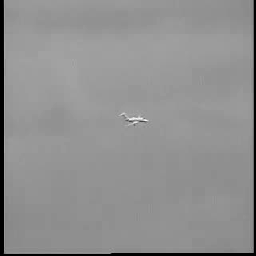
\includegraphics[width=0.35\textwidth]{./images/A1.png}}
    \phantom{123}
    \subfloat[测试集中的对应图像]{%
        
\includegraphics[width=0.35\textwidth]{./images/A1_y.png}}\\
%     \caption{同一图像的原始版本、测试集版本、训练集的多个变体}
%     \label{fig:datas}
% \end{figure}

% \begin{figure}[htbp]
% \ContinuedFloat
% \centering
    % \phantom{123}
    \subfloat[对应图像在训练集中的变体 1]{%
        
\includegraphics[width=0.35\textwidth]{./images/A1_x00.png}}
    \phantom{123}
    \subfloat[对应图像在训练集中的变体 2]{%
        
\includegraphics[width=0.35\textwidth]{./images/A1_x01.png}}\\
    % \phantom{123}
    \subfloat[对应图像在训练集中的变体 3]{%
        
\includegraphics[width=0.35\textwidth]{./images/A1_x02.png}}
    \phantom{123}
    \subfloat[对应图像在训练集中的变体 4]{%
        
\includegraphics[width=0.35\textwidth]{./images/A1_x03.png}}\\
    \caption{同一图像的原始版本、测试集版本、训练集的多个变体}
    \label{fig:datas}
\end{figure}

\newpage
\subsection{确定网络架构}

鉴于本次所给数据不同类别之间特征区分较为明显,因此使用的网络架构越简单越好。本实验中直接采用最简单多层感知器模型,模型架构见图 \ref{fig:perceptron}。

输入层的节点数是 $10\times10=100$。

输出层的节点数是 $4$。

由于此次数据分类任务较为简单,因此一层隐藏层就足够满足我们的要求。隐藏层的节点数也不用太多,目的是提高性能,也避免过拟合。单层隐藏层的节点数一般满足下面的经验公式,可以使网络的准确率与通用性达到较好的平衡:
$$\text{隐藏层节点数}=k\times\sqrt{\text{输入层节点数}+\text{输出层节点数}}$$

这里的 $k$ 是一个常数,范围取 $[0.3, 3]$ 为宜。

本次实验的单层隐藏层节点数取 5。

\def\incnt{4}
\def\midcnt{5}
\def\outcnt{4}
\tikzset{%
  every neuron/.style={
    circle,
    draw,
    minimum size=1cm
  },
  neuron missing/.style={
    draw=none,
    scale=2.8,
    text height=0.333cm,
    execute at begin node=\color{black}$\vdots$
  },
}
\begin{figure}[htbp]
\centering
\begin{tikzpicture}[x=1.5cm, y=1.5cm, >=stealth,shorten >=2pt, shorten <=2pt, scale=0.7]
    \foreach \m/\l [count=\y] in {1,2,3,missing,4}
      \node [every neuron/.try, neuron \m/.try] (input-\m) at (0,2.5-\y) {};
    \foreach \m [count=\y] in {1,missing,2}
      \node [every neuron/.try, neuron \m/.try ] (hidden-\m) at (3,2-\y*1.25) {};
    \foreach \m [count=\y] in {1,missing,2}
      \node [every neuron/.try, neuron \m/.try ] (output-\m) at (6,1.5-\y) {};
    \foreach \l [count=\i] in {1,2,3,m}
      \draw [stealth-] (input-\i) -- ++(-1.5,0)
        node [above, midway] {$i_\l$};
    % \foreach \l [count=\i] in {1,n}
    %   \node [above] at (hidden-\i.north) {$H_\l$};
    \foreach \l [count=\i] in {1,n}
      \draw [->] (output-\i) -- ++(1,0)
        node [above, midway] {$o_\l$};
    \foreach \i in {1,...,4}
      \foreach \j in {1,...,2}
        \draw [->] (input-\i) -- (hidden-\j);
    \foreach \i in {1,...,2}
      \foreach \j in {1,...,2}
        \draw [->] (hidden-\i) -- (output-\j);
    \foreach \l [count=\x from 0] in {输入, 隐藏, 输出}
      \node [align=center, above] at (\x*3,2) {\l 层};
\end{tikzpicture}
\caption{本次实验采取的神经网络架构:只有一层隐藏层的感知器}
\label{fig:perceptron}
\end{figure}

\subsection{实现网络主体并进行训练}

\subsubsection{前向传播}
前向传播,其实就是网络根据输入层的数据以及权重和偏置,计算得到输出层的过程。

后一层节点的值由前一层的节点值以及权重和偏置计算得出,最后再通过一个激活函数的映射。示意图见图 \ref{fig:forward}。

这一步可以抽象表示为:$$N_{i+1} = f(W_i,B_i,N_{i})$$

其中,$N_i$ 为第 $i$ 层节点的值,$W_i$ 为连接第 $i$ 层和第 $i+1$ 层节点的权重矩阵,$B_i$ 为连接第 $i$ 层和第 $i+1$ 层节点的偏置矩阵,$f$ 为激活函数。

本次实验采用的激活函数 $f$ 为 Sigmoid 函数,其表达式为:$$S(x) = \frac{e^x}{e^x+1}$$

\begin{figure}[htbp]
\centering
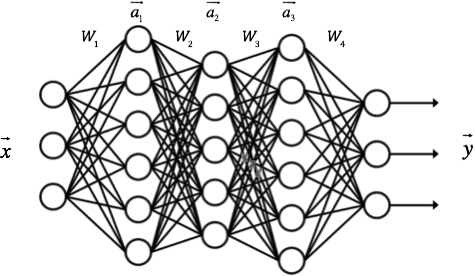
\includegraphics[width=0.6\textwidth]{images/forward.png}
\caption{前向传播的示意图}
\label{fig:forward}
\end{figure}

\subsubsection{后向传播}

后向传播包含两部分,误差计算和权重更新。由于是从输出层开始从后向前进行计算,因此称为后向传播。示意图见图 \ref{fig:back}。

对于输出层节点 $i$,误差可由下式计算得到:
$$\delta_i = y_i (1-y_i)(t_i-y_i)$$

其中,$\delta_i$ 是节点 $i$ 的误差,$y_i$ 是节点 $i$ 的输出,$t_i$ 是样本对应于节点 $i$ 的目标值。

对于隐藏层节点 $i$,误差可由下式计算得到:
$$\delta_i = y_i (1-y_i) \sum_k w_{ki}\delta_k$$

其中,$\delta_i$ 是节点 $i$ 的误差,$y_i$ 是节点 $i$ 的输出,$w_{ki}$ 是节点 $i$ 到它的下一层节点 $k$ 的连接的权重,$\delta_k$ 是节点 $i$ 的下一层节点 $k$ 的误差。

权重的更新遵循下式:
$$w_{ji} \leftarrow w{ji} + \eta \delta_j x_{ji}$$

其中,$w_{ji}$ 是节点 $i$ 到节点 $j$ 的权重,$\eta$ 为学习率,本实验中选取为常数 0.1,$\delta_j$ 是节点 $j$ 的误差,$x_{ji}$ 是节点 $i$ 传递给节点 $j$ 的输入。

偏置的更新遵循下式:
$$b_{ji} \leftarrow b{ji} + \eta \delta_j$$
其中,$b_{ji}$ 是节点 $i$ 到节点 $j$ 的偏置,$\eta$ 为学习率,$\delta_j$ 是节点 $j$ 的误差。

\begin{figure}[htbp]
\centering
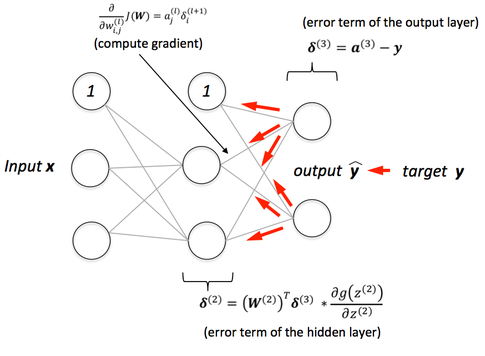
\includegraphics[width=0.8\textwidth]{images/back.png}
\caption{后向传播的示意图}
\label{fig:back}
\end{figure}

\newpage

\subsection{优化超参数}

经过上述步骤,就可以完成网络的训练了。只是相关的超参数,即网络的层数、各隐藏层的节点数、权重和偏置的初始化范围以及学习率等等,都需要适当的优化,才能使网络达到最佳的性能。

常用的超参数优化方式,包括网格搜索法、随机采样法、穷举法、贝叶斯优化法,以及最简单的手动调试法。

这其实也是一个较大的课题,只是与本次实验关联较小,因此这里不多加叙述。

\subsection{测试数据}

训练好网络以后,就需要将训练好的网络结构以及对应的权重和偏置应用到测试集中。这一步和网络训练过程中的前向传播较为相似,不再赘述。


\newpage

\section{代码实现}
\subsection{文件预处理}
限于篇幅,这里略去了部分细节,完整的代码请见附件。

重命名文件这一步对算法本身没有作用,只是为了后面方便对比分类结果和真实结果。

\begin{lstlisting}[style=myPython,caption={重命名文件}]
def renameFiles():
    if os.path.exists(data_renamed): 
        shutil.rmtree(data_renamed)
    os.mkdir(data_renamed)

    for filename in os.listdir(data_original):
        name, ext = os.path.splitext(filename)
        # print(name)
        if ext == ".bmp":
            cls = "A"
        elif ext == ".png":
            cls = "B"
        elif ext == ".jpg":
            if name == "timg":
                cls = "D"
            else:
                cls = "C"
        else:
            cls = "X"
        shutil.copyfile(data_original+filename,data_renamed+cls+filename)
\end{lstlisting}

\subsection{生成训练集}
生成训练集,并将其导出到文件中,用于后续训练神经网络。

\begin{lstlisting}[style=myPython,caption={生成训练集}]
def onehot(idx,len):
    tmp = np.zeros(len)
    tmp[idx] = 1
    return tmp

def generateTrainData():
    if os.path.exists(data_train): 
        shutil.rmtree(data_train)
    os.mkdir(data_train)

    names,imgxs,labels,targets = [],[],[],[]
    for filename in os.listdir(data_renamed):
        print(">>> Generating train data for {}".format(filename))
        if filename[0] == "D":
            aug_num = 500
        else:
            aug_num = 4
        for i in range(aug_num):
            # name
            body, ext = os.path.splitext(filename)
            name = data_train+body+"_x{:0>2}".format(i)+ext
            names.append(name)
            # imgx
            imgx = cv2.imread(data_renamed+filename,0)
            imgx = cv2.resize(imgx,imgx_size)
            noise = noise_max * np.random.rand(imgx_size[0],imgx_size[1])
            imgx = imgx + noise
            cv2.imwrite(name,imgx)
            imgx = imgx/255
            imgx = imgx.flatten()
            imgxs.append(imgx)
            # label
            label = ord(filename[0])-ord("A")
            labels.append(label)
            # target
            target = onehot(label,label_size)
            targets.append(target)

    # dump train data
    with open(dumped_train_data, "wb") as wf:
        pickle.dump([names,imgxs,labels,targets], wf)
\end{lstlisting}

\subsection{生成测试集}
生成测试集,并导出到文件中,用于后续测试神经网络的性能和准确率,

\begin{lstlisting}[style=myPython,caption={生成测试集}]
def generateTestData():
    if os.path.exists(data_test): 
        shutil.rmtree(data_test)
    os.mkdir(data_test)
    names,imgxs,labels,targets = [],[],[],[]
    for filename in os.listdir(data_renamed):
        # name
        body, ext = os.path.splitext(filename)
        name = data_test+body+"_y"+ext
        names.append(name)
        # imgx
        imgx = cv2.imread(data_renamed+filename,0)
        imgx = cv2.resize(imgx,imgx_size)
        cv2.imwrite(name,imgx)
        imgx = imgx/255
        imgx = imgx.flatten()
        imgxs.append(imgx)
        # label
        label = ord(filename[0])-ord("A")
        labels.append(label)
        # target
        target = onehot(label,label_size)
        targets.append(target[np.newaxis])

    # dump test data
    with open(dumped_test_data, "wb") as wf:
        pickle.dump([names,imgxs,labels,targets], wf)
\end{lstlisting}

\subsection{训练神经网络}
训练神经网络,包含前向传播和后向传播两个部分。这里使用向量化编程的思想,显著提高了算法的运行速度。

\begin{lstlisting}[style=myPython,caption={训练神经网络}]
weights = []
biases = []
def trainNetwork():
    global weights, biases

    # load imgxs and labels
    with open(dumped_train_data, "rb") as rf:
        names,imgxs,labels,targets = pickle.load(rf)

    # initialize weights and biases
    for i in range(layer_num-1):
        weights.append(np.random.rand(node_nums[i],node_nums[i+1]) * wran)
        biases.append(np.zeros((1,node_nums[i+1])))

    accuracies = []
    # train through all samples
    for h in range(epochs):
        tic = time.time()
        total_count = len(imgxs)
        wrong_count = 0
        for i in range(len(imgxs)):
            is_wrong = trainSingleSample(names[i],imgxs[i], labels[i], targets[i])
            wrong_count += is_wrong
        toc = time.time()
        accuracy = round(100*(1-wrong_count/total_count),2)
        accuracies.append(accuracy)
        print("Epoch:{} == Time: {} s == Accuracy:{}/{}={}%".format(h,round(toc-tic,3),total_count-wrong_count,total_count,accuracy))
    plt.plot(list(range(len(accuracies))),accuracies)
    plt.ylabel("Accuracy of training data")
    plt.xlabel("Epoch")
    plt.show()

    # dump weights and biases
    with open(dumped_weights, "wb") as wf:
        pickle.dump([node_nums,layer_num,weights,biases], wf)

def nsigmoid(x):
    return 1 / (1+math.exp(-x))
sigmoid = np.vectorize(nsigmoid)

def trainSingleSample(name, imgx, label, target):
    global weights, biases
    # Initialize nodes vales
    nodes = []
    deltas = []
    for i in range(layer_num):
        nodes.append(np.zeros((1,node_nums[i])))
        deltas.append(np.zeros((1,node_nums[i])))
    nodes[0] = imgx[np.newaxis]

    # forward propagation
    for i in range(layer_num-1):
        nodes[i+1] = sigmoid(np.matmul(nodes[i], weights[i]) + biases[i])

    # calculate deltas
    for i in range(layer_num)[::-1]:
        if i == layer_num-1: # ouput layer
            deltas[i] = nodes[i]*(1-nodes[i])*(target-nodes[i])
        else: # hidden layer
            dtmp = np.matmul(weights[i],deltas[i+1].T)
            deltas[i] = nodes[i]*(1-nodes[i])*(dtmp.T)

    # update weights
    for i in range(layer_num-1):
        weights[i] += step * np.matmul(nodes[i].T, deltas[i+1])
        biases[i] += step * deltas[i+1]

    # check output label
    if np.argmax(nodes[-1]) == label:
        is_wrong = 0
    else:
        is_wrong = 1
    return is_wrong
\end{lstlisting}

\subsection{测试神经网络}
测试神经网络,并输出准确率的结果。

\begin{lstlisting}[style=myPython,caption={测试神经网络}]
def testNetwork():
    # load test data
    with open(dumped_test_data, "rb") as rf:
        names,imgxs,labels,targets = pickle.load(rf)
    # load trained weights
    with open(dumped_weights, "rb") as rf:
        node_nums,layer_num,weights,biases = pickle.load(rf)
    # test data
    total_count = len(imgxs)
    wrong_count = 0
    tic = time.time()
    for i in range(len(imgxs)):
        name,imgx,label,target = names[i],imgxs[i], labels[i], targets[i]
        # Initialize nodes vales
        nodes = []
        for i in range(layer_num):
            nodes.append(np.zeros((1,node_nums[i])))
        nodes[0] = imgx[np.newaxis]
        # forward propagation
        for i in range(layer_num-1):
            nodes[i+1] = np.matmul(nodes[i], weights[i]) + biases[i]
            nodes[i+1] = sigmoid(nodes[i+1])
        # check output label
        if np.argmax(nodes[-1]) == label:
            is_wrong = 0
        else:
            is_wrong = 1
            wrong_count += 1
            # print(name)
    toc = time.time()
    print("Time: {} s -- Accuracy:{}/{}={}%".format(round(toc-tic,3),total_count-wrong_count,total_count,round(100*(1-wrong_count/total_count),2)))
\end{lstlisting}

\newpage

\section{结果与分析}
\subsection{训练结果}

神经网络训练过程中的准确率变化如图 \ref{fig:train} 所示。

\begin{figure}[htbp]
\centering
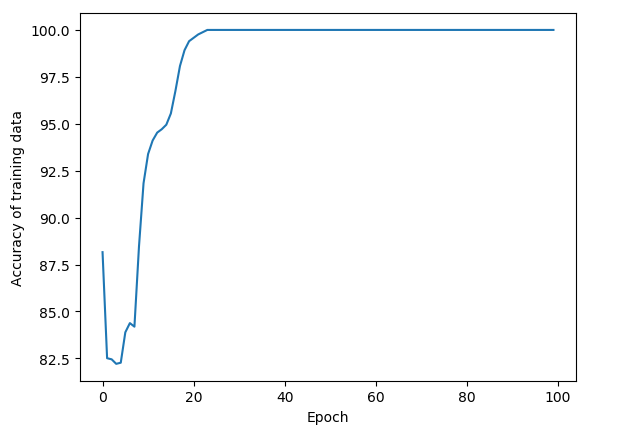
\includegraphics[width=\textwidth]{images/train.png}
\caption{神经网络的训练准确率曲线}
\label{fig:train}
\end{figure}

从图中可以看出:
\begin{enumerate}[leftmargin=*,labelindent=2em]
\item 第 1 次迭代就已经有了较高的准确率(约为88\%),说明生成的训练集数量充足,经过一次迭代就已经使网络的权重达到较佳的状态
\item 前几次迭代中,准确率出现了微小的波动,说明此时网络还未到达较为稳定的状态,部分训练数据对网络的泛化造成了一定的影响
\item 在几次迭代以后,准确率稳步上升,并且最终到达 100\%,说明网络训练状况优良,训练算法较好
\item 大约 25 次左右的迭代,就已经能达到 100\% 的准确率,并且保持稳定,表明我们的学习率选取得较为合适,使得权重收敛状况较好,也从侧面体现了轻量级网络训练较快的优点
\end{enumerate}

\vspace{0.5\baselineskip}
命令行的输出如下:
\begin{itemize}[label={},leftmargin=2em]
\item \begin{lstlisting}[style=plainText,caption={训练过程中的输出}]
Epoch:0 == Time: 0.102 s == Accuracy:1467/1664=88.16%
Epoch:1 == Time: 0.103 s == Accuracy:1373/1664=82.51%
Epoch:2 == Time: 0.112 s == Accuracy:1372/1664=82.45%
Epoch:3 == Time: 0.104 s == Accuracy:1368/1664=82.21%
Epoch:4 == Time: 0.103 s == Accuracy:1369/1664=82.27%
Epoch:5 == Time: 0.103 s == Accuracy:1396/1664=83.89%
Epoch:6 == Time: 0.106 s == Accuracy:1404/1664=84.38%
Epoch:7 == Time: 0.106 s == Accuracy:1401/1664=84.19%
Epoch:8 == Time: 0.104 s == Accuracy:1472/1664=88.46%
Epoch:9 == Time: 0.106 s == Accuracy:1528/1664=91.83%
Epoch:10 == Time: 0.104 s == Accuracy:1554/1664=93.39%
Epoch:11 == Time: 0.106 s == Accuracy:1566/1664=94.11%
Epoch:12 == Time: 0.108 s == Accuracy:1573/1664=94.53%
Epoch:13 == Time: 0.11 s == Accuracy:1576/1664=94.71%
Epoch:14 == Time: 0.107 s == Accuracy:1580/1664=94.95%
Epoch:15 == Time: 0.106 s == Accuracy:1590/1664=95.55%
Epoch:16 == Time: 0.106 s == Accuracy:1610/1664=96.75%
Epoch:17 == Time: 0.106 s == Accuracy:1632/1664=98.08%
Epoch:18 == Time: 0.103 s == Accuracy:1646/1664=98.92%
Epoch:19 == Time: 0.103 s == Accuracy:1654/1664=99.4%
Epoch:20 == Time: 0.105 s == Accuracy:1657/1664=99.58%
Epoch:21 == Time: 0.105 s == Accuracy:1660/1664=99.76%
Epoch:22 == Time: 0.104 s == Accuracy:1662/1664=99.88%
Epoch:23 == Time: 0.106 s == Accuracy:1664/1664=100.0%
Epoch:24 == Time: 0.105 s == Accuracy:1664/1664=100.0%
Epoch:25 == Time: 0.111 s == Accuracy:1664/1664=100.0%
Epoch:26 == Time: 0.106 s == Accuracy:1664/1664=100.0%
...
Epoch:99 == Time: 0.104 s == Accuracy:1664/1664=100.0%
\end{lstlisting}
\end{itemize}

\subsection{测试结果}
测试结果的命令行输出如下所示。

\begin{itemize}[label={},leftmargin=2em]
\item \begin{lstlisting}[style=plainText,caption={测试结果的输出}]
Time: 0.015 s
Accuracy:292/292=100.0%
\end{lstlisting}
\end{itemize}

从测试结果的输出中可以看到,即使训练集和测试集并不相同,但是我们的网络还是能达到 100\% 的准确率,也就是说,网络依旧能识别出不同类别图像的特征,体现了该网络模型较好的通用性。

此外,分类速度也很快,说明我们的网络性能较好,可以在短时间内处理大量的数据。

\newpage

\section{参考文献}

\begin{enumerate}
\item Wikipedia contributors. (2019, May 29). Artificial neural network. In Wikipedia, The Free Encyclopedia. Retrieved 18:24, May 30, 2019, from \url{https://en.wikipedia.org/w/index.php?title=Artificial_neural_network&oldid=899409597}

\item Wikipedia contributors. (2019, May 8). Hyperparameter optimization. In Wikipedia, The Free Encyclopedia. Retrieved 18:22, May 30, 2019, from \url{https://en.wikipedia.org/w/index.php?title=Hyperparameter_optimization&oldid=896193455}

\item Wikipedia contributors. (2019, May 19). Backpropagation. In Wikipedia, The Free Encyclopedia. Retrieved 18:23, May 30, 2019, from \url{https://en.wikipedia.org/w/index.php?title=Backpropagation&oldid=897855738}

\item Wikipedia contributors. (2019, May 25). Multilayer perceptron. In Wikipedia, The Free Encyclopedia. Retrieved 18:24, May 30, 2019, from \url{https://en.wikipedia.org/w/index.php?title=Multilayer_perceptron&oldid=898748424}

\item Stéfan van der Walt, S. Chris Colbert and Gaël Varoquaux. The NumPy Array: A Structure for Efficient Numerical Computation, Computing in Science \& Engineering, 13, 22-30 (2011), DOI:10.1109/MCSE.2011.37
\end{enumerate}

\end{document}